\documentclass{article}
\PassOptionsToPackage{hyphens}{url}\usepackage{hyperref}
\usepackage{listings}
\usepackage{graphicx}
\begin{document}
\noindent
Andreas Landgrebe\\
Computer Science 220\\
Lab 6: Haskell\\
\\
\\
\textbf{Questions}
\begin{enumerate}
\item Is Haskell a strongly-typed language? (You might want to review the definition and say a few words about how Haskell meets, or fails to meet the definition.) If you have trouble, you may look for Web resources to help you answer, but be sure to cite them.
\\
\\
Haskell is a strongly-typed language. This is the case because it is not possible for the programmer to work around the restrictions imposed by the type system. An example of a weak-typed language is C. This is the case because any pointer type is convertible to any other pointer type by casting.
\\
The following information was found on this website.

\url{http://stackoverflow.com/questions/2690544/what-is-the-difference-between-a-strongly-typed-language-and-a-statically-typed}

\item Haskell exhibits "referential transparency,” an idea that was mentioned in our book back in
chapter 6 (p. 225). Can you explain “referential transparency” in your own words or with an
example? (If you can’t, can you find—and cite—a good definition and/or example from the
Web different from the one in the Haskell tutorial I’ve asked you to read.)
\\
\\
The following definition was found on this website.
\\
\url{https://wiki.haskell.org/Referential_transparency}
\\
Referential transparency is a is a property that makes it easier to reason about the behavior of programs. This usually means that an expression can evaluate to the same result in any context. 
\\
\item Haskell has multiple exponentiation operators. Look them up, explain their differences, and
give examples
\\
The following explanation was found on the following website:
\\
\url{http://stackoverflow.com/questions/6400568/exponentiation-in-haskell}
\\
\begin{lstlisting}
There are three exponentiation operators. 
^, ^^ and **.
 ^ is non-negative integral exponentiation, 
 ^^ is integer exponentiation, 
 and ** is floating-point exponentiation. 
 Below are examples:
(^) :: (Num a, Integral b) => a -> b -> a
(^^) :: (Fractional a, Integral b) => a -> b -> a
(**) :: Floating a => a -> a -> a
\end{lstlisting}

\item Is there a clear operator precedence? Try to construct an operator precedence for at least the
arithmetic and relational and boolean operators. Either find this somewhere (and cite it) or
determine it through experimentation. (Remember about the parentheses around negative
constants! What happens if you leave them out?)
\\
The following information was found through this website.
\url{https://www.haskell.org/onlinereport/decls.html}
\\
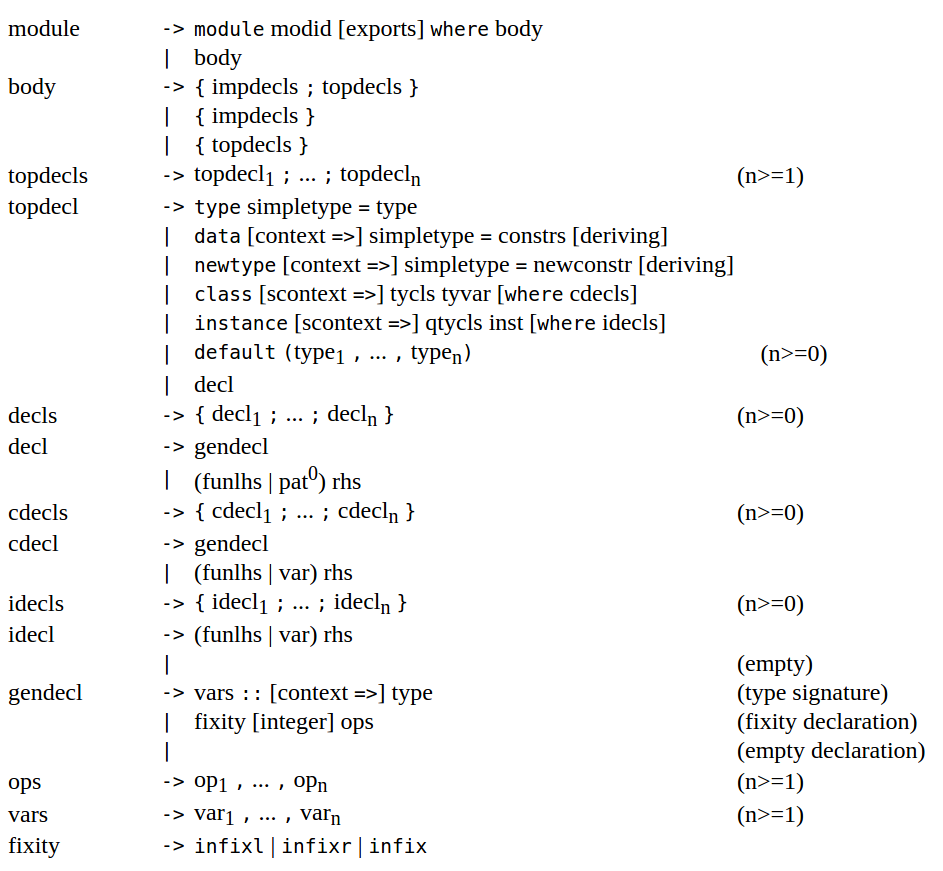
\includegraphics[scale=0.45]{Screenshot}
\newpage
\item How do lists in Haskell differ from lists in Python? (This is vague, but there should be at
least one very clear difference.)
\\
Lists in Haskell differ from lists in Python due to the fact that Python's list comprehension is taken directly from Haskell. The following information was found on this website.
\url{https://wiki.python.org/moin/PythonVsHaskell}
\\
\item Given your very limited experience with Haskell in the tutorial, what aspects of Haskell (so
far) do you find . . .
\begin{itemize}
\item the most interesting or unusual?
\\
The most interesting aspect of Haskell being able to import specific list to the graphical user interface in the terminal. 
\\
\item the hardest to understand?
\\
The hardest to understand is being able to understand the syntax of Haskell.
\\
\item the most frustrating?
\\
The most frustrating is realize that tabs and indexes make a substantial difference just like in Python. I didn't realize this until later on.
\\
\item the most fun?
\\
The most fun is realizing how less verbose this language compared to Java.
\end{itemize}
\end{enumerate}
\end{document}